\documentclass{article}
\usepackage{graphicx}
\usepackage{amsmath}
\usepackage{amssymb}
\usepackage{natbib}
\renewcommand{\refname}{References}
\usepackage{url}

\title{A Differential Geometric Approach to Economic Forecast}

\author{Babak Emami}

\date{\today}

\begin{document}
\maketitle

\begin{abstract}


\end{abstract}

\section{Introduction}\label{section:introduction}

The usual approach to predicting price of an asset is to regress the
historical prices of tat asset against a set of economic
indicators. The problem with this approach is that we still need
knowldege of the future values of economic indicators. This is done by
relying on estimate forecasts of econimic indicators which are often
based on qualitative methods, such as those in Blue Chip Economic
Indicators and Blue Chip Financial Forecasts~\cite{ref:blue-chip}. The
forecasts in Blue Chip publications are based on surveying top
business economists in the United States.

An approach is proposed to forecast economic variables without
depending on future values of any economic indicators. We look at the
economy as a multi-demensional manifold; each dimension is an economic
variable. These variables can be marco-economic indicators or asset
prices. We refer to this manifold as an economic universe. The
observed values of economic variables in a time period form a path in
this universe. We refer to this path as the economic path. We then
find a manifold for which this path is a geodesic, governed by a
system of differential equations. The fututre value of economc
variables can be predicted by solving this system of differential
equations.

In what follows the mathematical framework used is discussed and a
methodology is proposed to infer the structure of economic universe
given a set of observed economic variables.

\section{Mathematical Framework}\label{section:mathematical-framework}

Let us consider $n$ economic variables $x{1}$ to $x^{n}$ that are
smooth functions of time $t$; $x^{i} = x^{i}(t)$. Moreover, let us
consider a smooth real manifold $M$ equipped with
$(x^{1},x^{2},...,x^{n})$ as a coordinate system. Each set of
coordinate values $(x^{1}(t),...,x^{n}(t))$ denotes a point $p$ on
$M$. Values of these $n$ variables over a period of time $[0,T]$ form
a path over $M$. This path is smooth as $x^{i}$s are smooth functions
of time. Now let us add a constraint on $M$ by assuming that the path
formed by $x^{i}(t)$s is a geodesic of $M$. With this assumption, this
path is governed by the follwoing system of ordinary differential
equations,

\begin{equation}\label{eqn:geodesic}
\ddot{x}^{m} + \Gamma^{m}_{ab} \dot{x}^{a} \dot{x}^{b} = 0
\end{equation}

subject to,

\begin{equation}\label{eqn:geodesic-bc}
\dot{x}^{m}(0) = \dot{x}^{m}_{0}
\end{equation}

where $m,a,b \in [1,n] \cap \mathbb{N}$.

\section{Results}\label{section:results}

\section{Model Parameter Study}\label{section:model-parameter-study}

\begin{figure}\label{fig:tolerance-sensitivity-error}
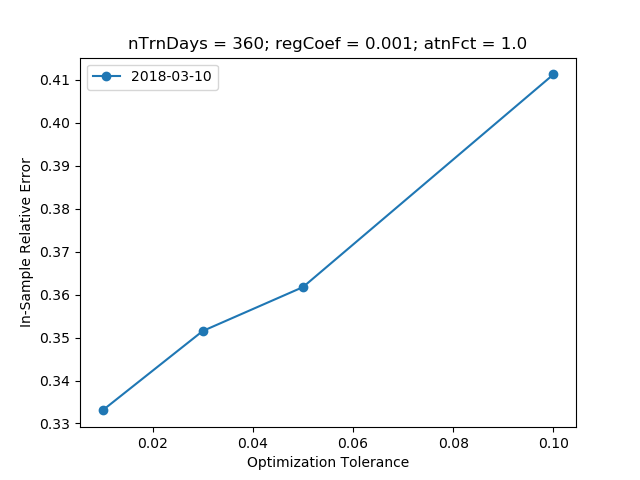
\includegraphics[bb=0 0 640 480]{figures/tolerance-sensitivity-error.png}
\caption{In-sample relative error vs. optimization tolerance.}
\end{figure}

\begin{figure}\label{fig:tolerance-sensitivity-oos-error}
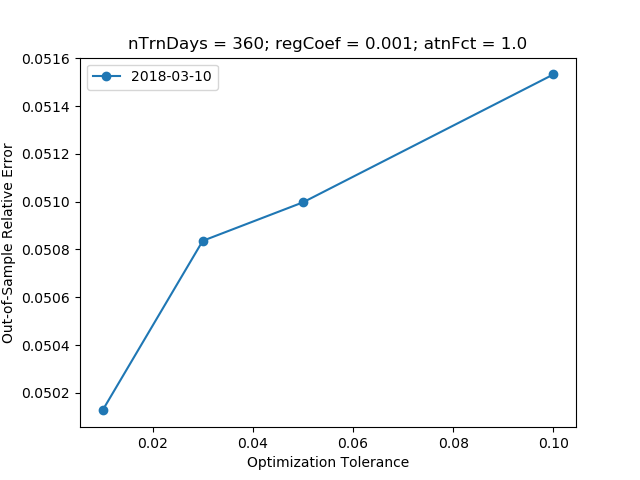
\includegraphics[bb=0 0 640 480]{figures/tolerance-sensitivity-oos-error.png}
\caption{Out-of-sample relative error vs. optimization tolerance.}
\end{figure}

\begin{figure}\label{fig:nTrnDays-sensitivity-error}
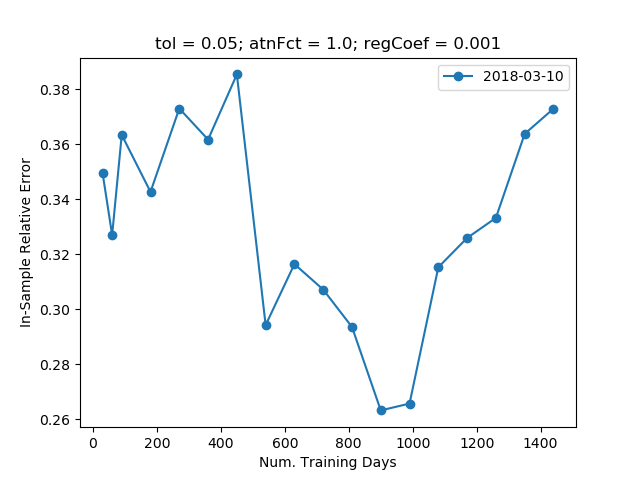
\includegraphics[bb=0 0 640 480]{figures/nTrnDays-sensitivity-error.png}
\caption{In-sample relative error vs. number of days used for training.}
\end{figure}

\begin{figure}\label{fig:nTrnDays-sensitivity-oos-error}
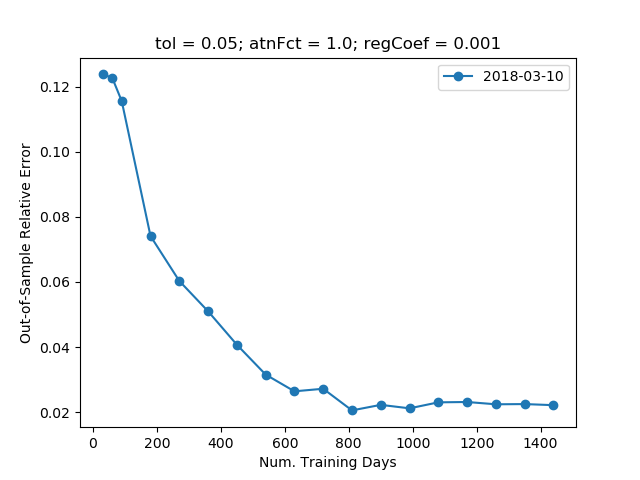
\includegraphics[bb=0 0 640 480]{figures/nTrnDays-sensitivity-oos-error.png}
\caption{Out-of-sample relative error vs. number of days used for training.}
\end{figure}

\begin{figure}\label{fig:regCoef-sensitivity-error}
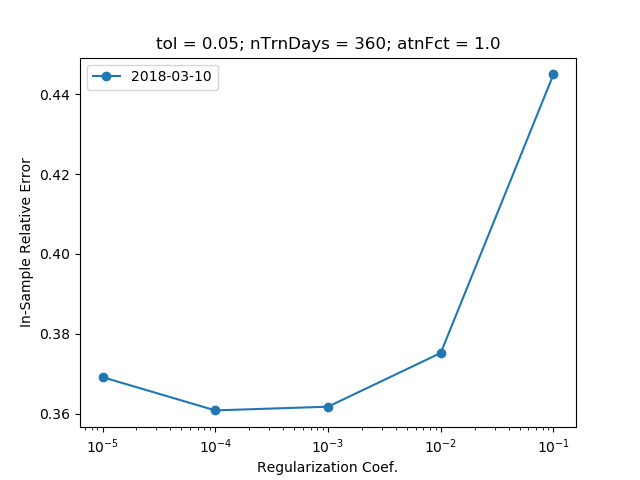
\includegraphics[bb=0 0 640 480]{figures/regCoef-sensitivity-error.png}
\caption{In-sample relative error vs. regularization coefficient.}
\end{figure}

\begin{figure}\label{fig:regCoef-sensitivity-oos-error}
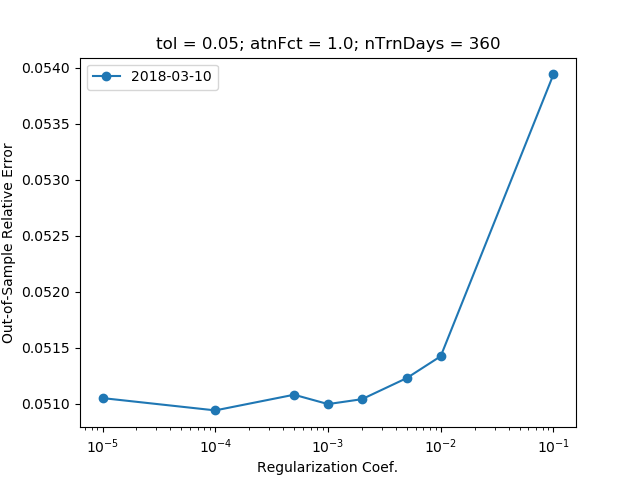
\includegraphics[bb=0 0 640 480]{figures/regCoef-sensitivity-oos-error.png}
\caption{Out-of-sample relative error vs. regularization coefficient.}
\end{figure}

\begin{figure}\label{fig:atnFct-sensitivity-error}
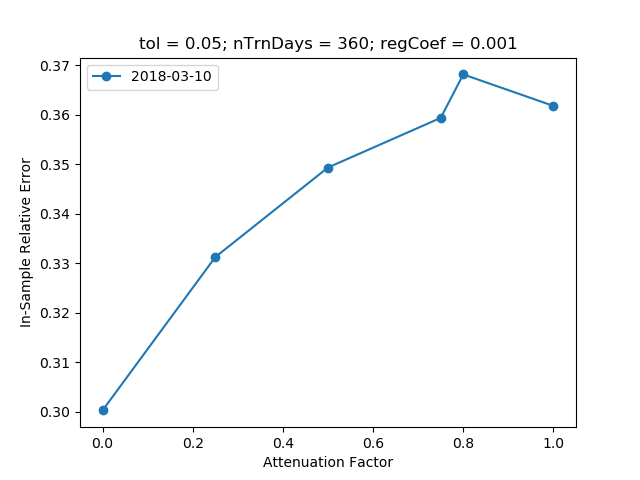
\includegraphics[bb=0 0 640 480]{figures/atnFct-sensitivity-error.png}
\caption{In-sample relative error vs. attenuation coefficient.}
\end{figure}

\begin{figure}\label{fig:atnFct-sensitivity-oos-error}
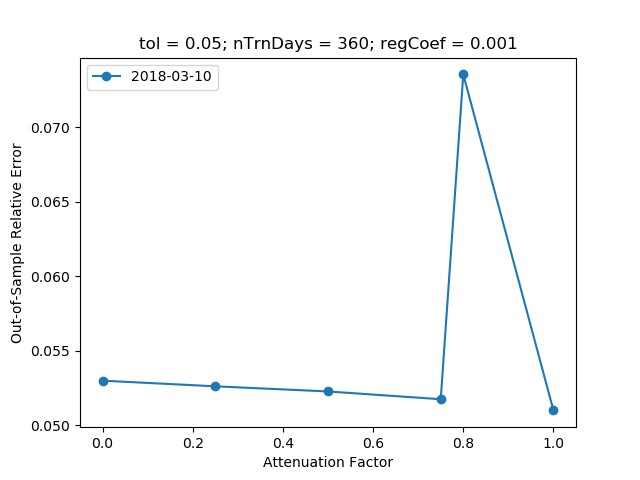
\includegraphics[bb=0 0 640 480]{figures/atnFct-sensitivity-oos-error.png}
\caption{Out-of-sample relative error vs. attenuation coefficient.}
\end{figure}

\begin{figure}\label{fig:gamma-time}
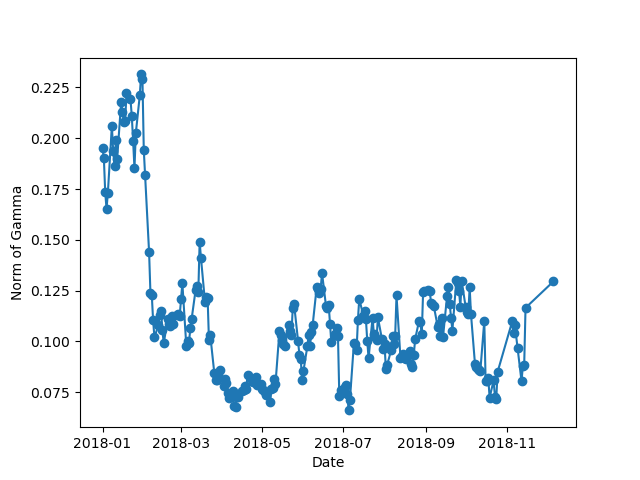
\includegraphics[bb=0 0 640 480]{figures/Gamma_time_2018.png}
\caption{Norm of Gamma vs. snapdate Each point on the plot comes from
  a model with a constant Christoffel symbol.}
\end{figure}

\section{Conclusions}\label{section:conclusions}

\bibliography{references}
\bibliographystyle{plain}

\end{document}

